\section{SUMBER-SUMBER DATA GEOSPASIAL}

Dalam dunia geospasial tidak jauh dengan data spasial. Data spasial ibarat hokum mutlak diperlukan dalam membuat peta atau melakukan analisis spasial. Namun kendalanya tidak semua data-data yang diperlukan tersedia. Dalam uraian berikut akan membahas sumber data spasial dari open geodata.
\begin{enumerate}
\item Ina Geoportal
Ina Geoportal adalah sumber data geospasial resmi untuk Indonesia yang  dibangun, dipelihara dan diawasi langsung oleh Badan Informasi Geospasial (BIG) yang di mana merupakan lembaga pemerintah yang bertanggung jawab penuh atas data geospasial nasional. Melalui Ina Geoportal ini kita dapat men-download data-data peta rupa bumi dalam skala 250 ribu, 50 ribu dan 25 ribu. Proses mendapatkan datanya pun cukup mudah, Kita hanya perlu mengisikan Nama, email, jenis data RBI, jenis pengguna dan terakhir tentu saja kita harus menyetujui ketentuan undang-undang yang berlaku. Pada gambar \ref{labelgambar1} merupakan tampilannya  
\begin{figure}[ht]
\centering
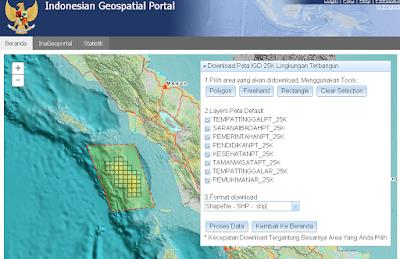
\includegraphics[width=0.5\textwidth]{pictures/ina_geospasial}
\caption{Ina Geoportal}
\label{labelgambar1}
\end{figure}

\item USGS Earth Explorer
USGS earth explorer merupakan sumber data spasial yang disediakan oleh lembaga survey geologi Amerika Serikat. Di earth explorer ini disediakan cukup banyak sekali data dengan berbagai macam tema, resolusi dan sensor, seperti citra satelit, Lidar, cuaca, radar, landcover dan lain sebagainya. Data-data tersedia umumnya mencakup data di wilayah Amerika. Namun, tidak hanya data-data tersebut yang tersedia melainkan data-data dengan cakupan global seperti data Digital Elevation Model (DEM), SRTM, citra satelit Landsat, monitoring vegetasi dan lain-lain.  Pada gambar \ref{labelgambar2} merupakan tampilannya  
\begin{figure}[ht]
\centering
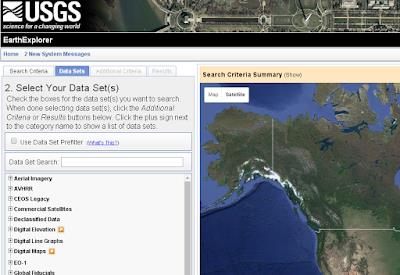
\includegraphics[width=0.5\textwidth]{pictures/usgs_earth_explorer}
\caption{USGS Earth Explorer}
\label{labelgambar2}
\end{figure}


\item Worldclim
Worldclim adalam sumber data geospasial yang menyediakan data curah hujan guna melakukan proses analisis spasial yang tersedia dalam format spasial. Worldclim menyuguhkan data curah hujan dan data iklim secara umum yang meliputi temperatur tahunan serta bulanan. Data ini diperoleh dari stasiun-stasiun cuaca di seluruh dunia yang dikumpulkan jadi satu dari tahun 1960-1990 (versi 1.4) dan 1970-2000 (versi 2). Data-data yang dikumpulkan kemudian diolah dan dianalisa sehingga dapat diprediksi data iklim untuk masa lalu, sekarang dan masa yang akan datang. Jadi, data ini bukan termasuk data realtime, akan tetapi analisa data iklim selama 30 tahun. Data wordclim dapat diperoleh dalam format raster dengan resolusi 1 km.  Pada gambar \ref{labelgambar3} merupakan tampilannya  

\begin{figure}[ht]
\centering
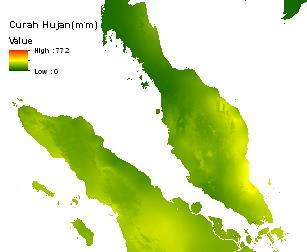
\includegraphics[width=0.5\textwidth]{pictures/data_worldclim}
\caption{USGS Data Worldclim}
\label{labelgambar3}
\end{figure}

\item Global Forest Change
Global Forest Change seperti merupakan data yang memonitor perubahan hutan. Data ini diperoleh dari analisis time series citra satelit Landsat mulai tahun 2000, dan terus diperbaharui secara berkala.  Sampai saat tulisan ini ditulis data yang tersedia sampai tahun 2014. Karena dianalisa dari data citra satelit Landsat maka data ini memiliki resolusi 30 meter, sehingga cocok untuk digunakan untuk analisa data dengan skala menengah. Data ini dikelola oleh Universitas Maryland Amerika Serikat. Cakupan data ini bersifat global dan dapat didownload dalam format “tif” dengan satu tile/scene berukuran 10 derajat x 10 derajat. Pada gambar \ref{labelgambar4} merupakan tampilannya
\begin{figure}[ht]
\centering
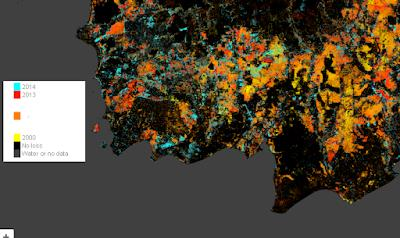
\includegraphics[width=0.5\textwidth]{pictures/Global_Forest_Change}
\caption{Global Forest Change}
\label{labelgambar4}
\end{figure}

\item Soil Grid
Soil Grid menyediakan informasi data tanah secara global. Karena sifatnya global tentu saja memiliki akurasi yang kasar dibandingkan dengan data jenis tanah dengan cakupan nasional atau provinsi. Data soil grid diperoleh dari analisa data-data tanah secara global yang diolah secara statisitk dengan metode kovarian dan regresi. Jenis tanah, kandungan carbon, air, gypsum dan lain-lain baik untuk tanah lapisan atas(top soil) maupun lapisan bawah (sub soil) adalah informasi yang dapat diperoleh dari Soil Grid. Data tersebut dapat didownload dalam format geotiff.  Pada gambar \ref{labelgambar5} merupakan tampilannya  

\begin{figure}[ht]
\centering
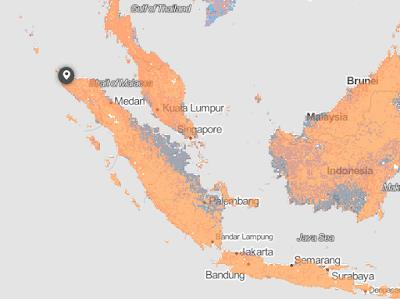
\includegraphics[width=0.5\textwidth]{pictures/Data_Tanah_Soil_Grid}
\caption{Data Tanah Soil Grid}
\label{labelgambar5}
\end{figure}

\item USGS GloVis
Sumber data geospasial yang menyediakan data geografis tentang bahaya alam yang mengancam kehidupan dan mata pencaharian, air, energi, mineral, dan sumber daya alam lainnya. Juga dampak kesehatan ekosistem dan lingkungan sekitar serta dampak perubahan iklim dan penggunaan lahan. Ilmuwan USGS GloVis sedang mengembangkan metode dan alat baru untuk memungkinkan informasi yang tepat waktu, relevan, dan berguna tentang Bumi dan prosesnya.  Pada gambar \ref{labelgambar6} merupakan tampilannya  

\begin{figure}[ht]
\centering
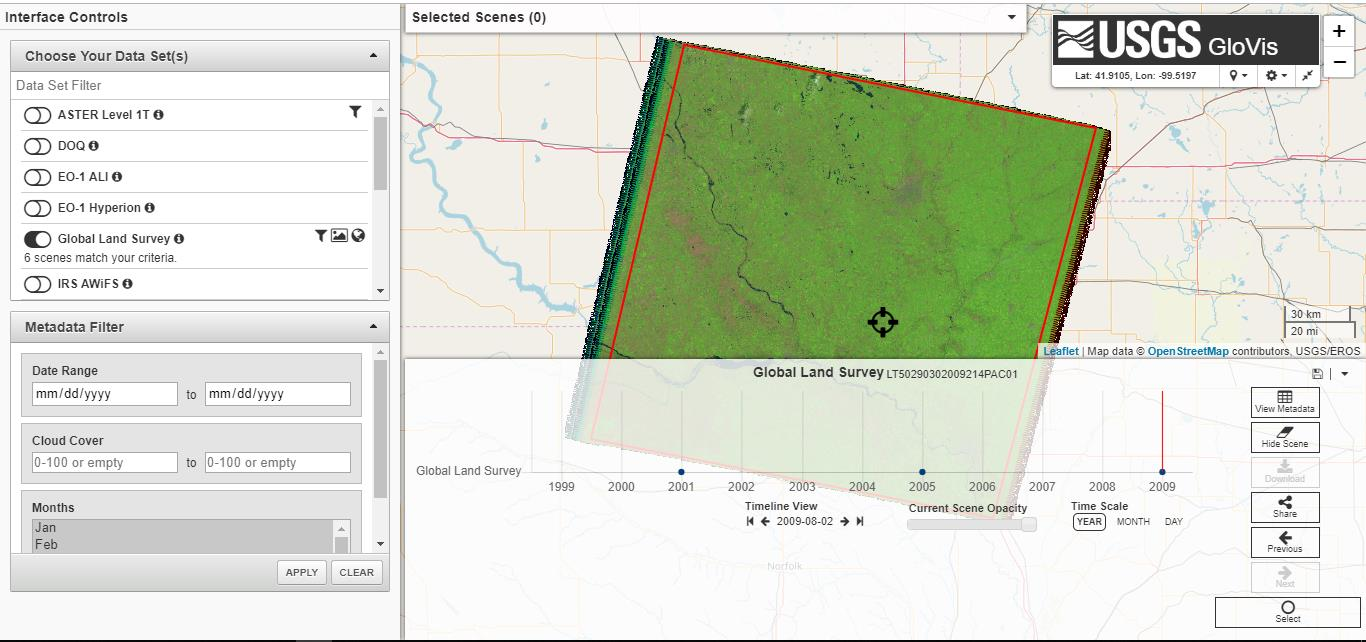
\includegraphics[width=0.5\textwidth]{pictures/USGS_GloVis}
\caption{USGS GloVis}
\label{labelgambar6}
\end{figure}

\item Theia- Land Data Center
Theia-Land Data Center adalah organisasi antar-lembaga nasional Prancis yang dirancang untuk mendorong penggunaan gambar yang didapatkan dari hasil pengamatan ruang permukaan tanah. Theia menawarkan komunitas ilmiah dan aktor kebijakan publik dari berbagai gambar di berbagai skala, metode dan layanan.  Pada gambar \ref{labelgambar7} merupakan tampilannya  
\begin{figure}[ht]
\centering
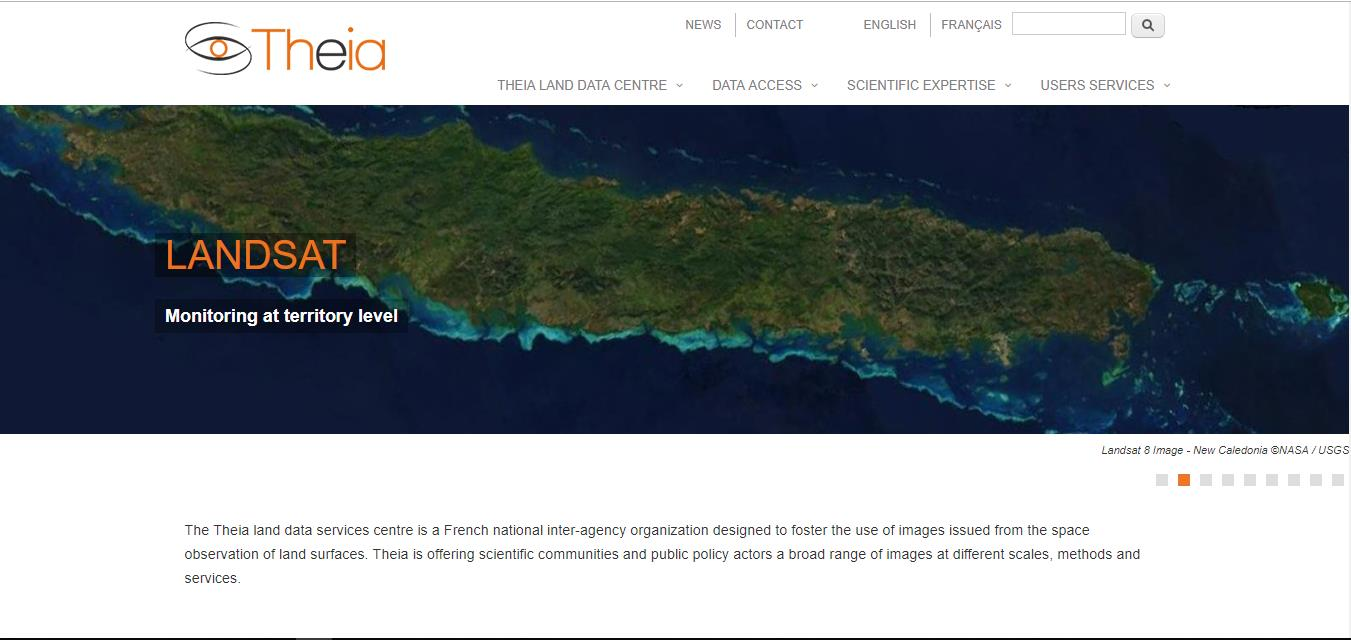
\includegraphics[width=0.5\textwidth]{pictures/Theia_Land_Data_Center}
\caption{Theia- Land Data Center}
\label{labelgambar7}
\end{figure}
\end{enumerate}